\section{Mason}

At the inception of the project, an initial focus was put towards experimentation. As the project continued this focus became balanced more evenly between empirical investigation and the engineering of the system itself, however at the outset it was evident that one of the multi-agent frameworks covered in Chapter \ref{ch:background} would be a solid foundation upon which to build the simulation.

MASON (Multi-Agent Simulation of Neighbourhoods, or Networks) is a versatile Java library for providing the key architecture in agent-based applications. MASON provides a range of environment representations, or \textit{fields} in MASON nomenclature, and a GUI system that intuitively visualises system components that interact in and with the MASON fields.

This project did not tie itself heavily to MASON's broad range of features. MASON only provided a very lightweight framework to act as a foundation for the simulation construction: MASON fundamentally revolves around a \texttt{Scheduler}, object. The Scheduler is a decorated priority queue. For an agent to act in the system it must inherit the \code{Steppable} interface, which guarantees the agent has a \code{step()} method. Agents are queued into the Scheduler for each time step, and the Scheduler executes the agent's step method when it reaches the top of the queue. In compliment with this simple functionality, the Scheduler will step higher priority agents first and will step agents of equal priority in a uniformly random order.

In addition to the Scheduler, MASON's other contribution to the project was providing a GUI, and MASON's GUI-compliant graph data structure functionality. MASON Networks are a simple collection of arbitrary user-defined objects to use as nodes, and a map between nodes and their associated Edge objects. While MASON expects users to provide a class to act as a node, it provides its own Edge class. Edge objects store a `from node', `to node' and an arbitrary user-defined child object, which is expected to store semantic data about what the Edge represents. MASON Networks hence act as wrappers for user-defined node and edge objects - to that end, \code{Junction} objects were defined as the Network's node objects, and \code{Road} objects were constructed to provide a semantic representation of roads in the simulation. The driving reason for using a MASON network rather than constructing a graph directly from the \code{Junction} and \code{Road} objects is the ease of the MASON network integration with MASON's own GUI and visualisation tools.


\section{System Overview}

At the highest level, the project is composed of a simulation package, and classes which leverage it. Figure \ref{fig:system_overview} gives a simple class-relationship diagram of the system which articulates this high-level split as well as portraying a lower level system composition; the simulation package consists of a set of agents, a collection of environment classes, a pair of classes for implementing the A* algorithm, and most importantly, the \code{CoreSimulation} class.

\begin{figure}
    \centering
    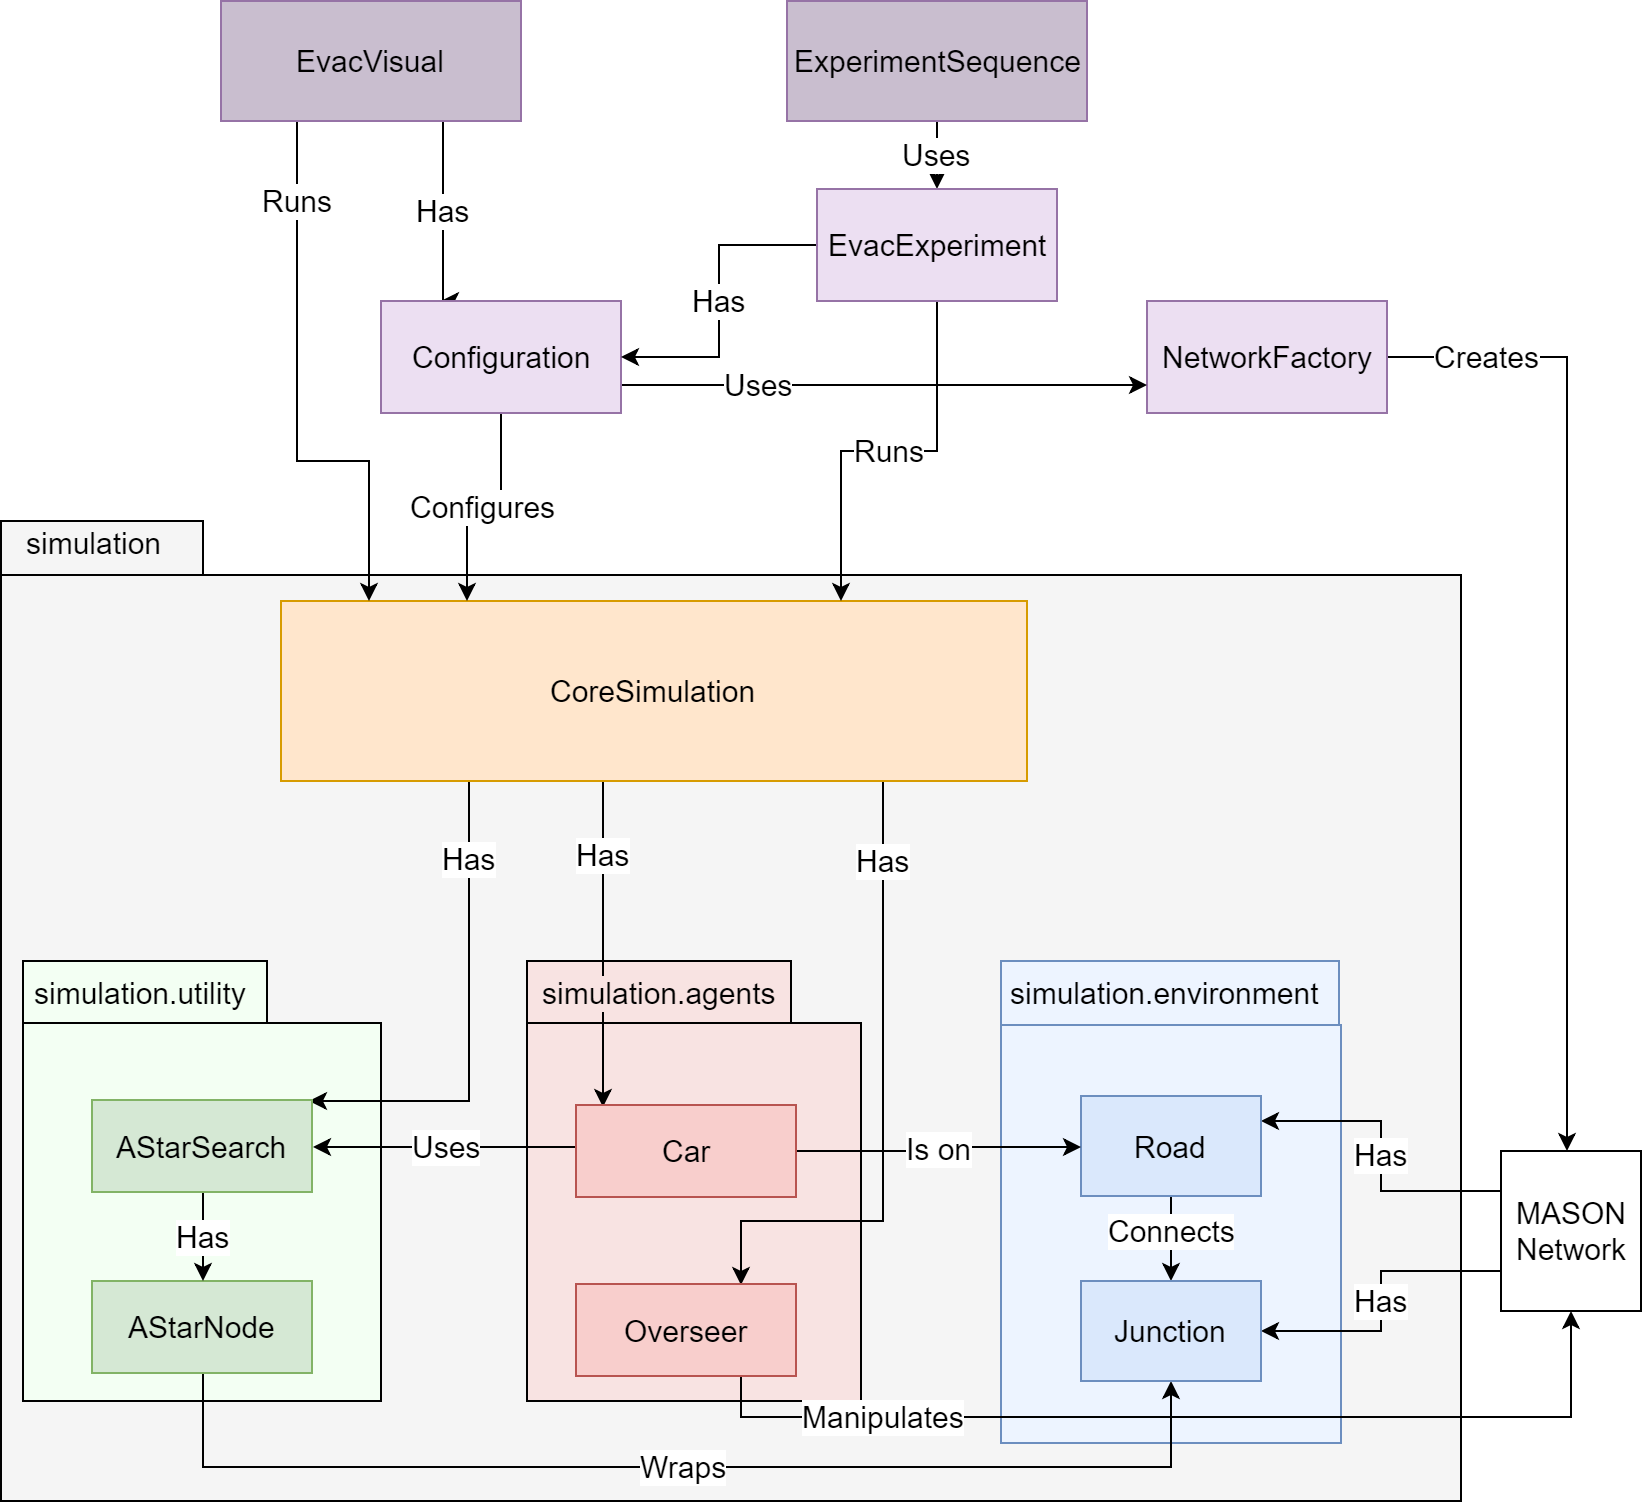
\includegraphics[width=0.95\linewidth]{images/system_overview.png}
    \caption{Project component relationship diagram}
    \label{fig:system_overview}
\end{figure}

TABLE OF CLASSES